\documentclass[conference,letterpaper]{IEEEtran}
\usepackage[utf8]{inputenc}
\usepackage[T1]{fontenc}
\usepackage{amsmath,amssymb}
\usepackage{graphicx}
\usepackage{booktabs}
\usepackage{multirow}
\usepackage{url}
\usepackage[hidelinks]{hyperref}
\usepackage{cite}

\renewcommand{\abstractname}{Resumen}
\renewcommand{\IEEEkeywordsname}{Palabras clave}
\renewcommand{\tablename}{TABLA}
\renewcommand{\figurename}{Fig.}
\renewcommand{\refname}{Referencias}
\renewcommand{\appendixname}{Anexo}
\def\IEEEtitletopspace{0.6in}

\begin{document}

\title{Predicción de fallas en una flota de máquinas mediante deep learning: modelo final, confiabilidad y política de mantenimiento}

\author{\IEEEauthorblockN{Luisa Merlo García, Edgar Osvaldo Navarro García, Ariana Guadalupe Rosales Villalobos}
\IEEEauthorblockA{Machine Learning y Deep Learning --- Tecnológico de Monterrey, Campus Guadalajara\\
Entrega 3 (final), 27 de noviembre de 2026}}

\maketitle

\begin{abstract}
Construimos un sistema de alerta temprana que estima, para cada una de 100 máquinas y cada hora, la probabilidad de que algún componente falle en las siguientes 24 horas y cuál será. Sobre el conjunto simulado Azure Predictive Maintenance, con partición temporal fija, comparamos líneas base clásicas (regresión logística y XGBoost, que con variables de ventana diseñadas a mano alcanza PR-AUC de 0.998 y con la serie cruda 0.887), redes secuenciales (LSTM, TCN, CNN-LSTM) y un codificador Transformer con token de máquina, todos alimentados con la misma serie cruda de 13 canales horarios. La TCN de la semana 2 (ventana de 24 h, sobremuestreo de ventanas pre-falla) quedó como modelo final por la regla de selección por costo definida antes de ver los resultados: el Transformer y un ensamble de cinco TCN empataron dentro de 1~\% del costo en validación. En el periodo de prueba (noviembre--diciembre de 2015), evaluado una sola vez, el modelo obtuvo PR-AUC de 0.996, anticipó las 121 fallas de componente con un aviso medio de 21 horas y generó 12 falsas alarmas (1.4 por semana para toda la flota). Con los costos del enunciado, la política basada en el modelo cuesta 2.2 millones al año (IC 95~\%: 1.9--2.5), contra 8.4 millones del reemplazo por calendario y 10.9 millones de operar hasta la falla. Los gradientes integrados muestran que cada componente se asocia con un sensor y uno o dos tipos de error, coherente con el análisis exploratorio.
\end{abstract}

\begin{IEEEkeywords}
mantenimiento predictivo, series de tiempo, TCN, Transformer, calibración, gradientes integrados, análisis de costo
\end{IEEEkeywords}

\section{Introducción}
Una falla no anticipada saca a la máquina de operación, moviliza al técnico de guardia y daña material en proceso. El objetivo del proyecto es pasar de una estrategia correctiva y por calendario a una predictiva: avisar con suficiente anticipación qué máquina va a fallar y en qué componente, para intervenirla en una ventana planeada. Siguiendo la perspectiva de planta del enunciado, juzgamos los modelos por las decisiones que permiten: fallas evitadas, falsas alarmas y horas de anticipación, y finalmente por el costo esperado.

Este reporte integra las tres semanas. La sección~\ref{sec:datos} resume los datos, las etiquetas y el control de fuga; la~\ref{sec:w1} la línea base; la~\ref{sec:w2} los modelos secuenciales; la~\ref{sec:w3} el modelo avanzado, la incertidumbre, la interpretabilidad y la política; la~\ref{sec:test} los resultados en prueba; y las secciones~\ref{sec:disc} y~\ref{sec:prod} la discusión, las limitaciones y lo que haría falta para producción.

\section{Datos, etiquetas y fuga de información}\label{sec:datos}
El conjunto Azure Predictive Maintenance~\cite{azure} contiene telemetría horaria de cuatro sensores (\textit{volt, rotate, pressure, vibration}) de 100 máquinas durante 2015 (876\,100 filas), 3\,919 errores no fatales de cinco tipos, 3\,286 reemplazos de componentes (desde 2014), 761 fallas de componente y el modelo y la antigüedad de cada máquina.

\textit{Etiquetas.} Para cada máquina $m$ y hora $t$, $y_{\text{bin}}=1$ si algún componente falla en $(t, t+24\,\text{h}]$; la etiqueta multiclase es el componente con la falla más próxima en esa ventana (0 si ninguno). El intervalo excluye $t$, así que la hora de la falla no se etiqueta a sí misma.

\textit{Partición.} Entrenamiento: horas del 1 de enero al 30 de agosto; validación: 1 de septiembre al 30 de octubre; prueba: 1 de noviembre al 31 de diciembre. Se deja un margen de 24~h antes de cada frontera para que ninguna etiqueta dependa de fallas posteriores al periodo. La Tabla~\ref{tab:desbalance} muestra el desbalance: menos de 2.1~\% de horas positivas, por lo que no reportamos exactitud.

\begin{table}[t]
\centering
\caption{Desbalance por conjunto (\% de horas positivas)}
\label{tab:desbalance}
\begin{tabular}{lrrrrrr}
\toprule
Conjunto & Horas & Pos. & comp1 & comp2 & comp3 & comp4 \\
\midrule
Entren. & 580\,200 & 2.02 & 0.58 & 0.69 & 0.37 & 0.50 \\
Valid. & 144\,000 & 1.84 & 0.35 & 0.75 & 0.33 & 0.50 \\
Prueba & 146\,400 & 1.83 & 0.49 & 0.73 & 0.30 & 0.41 \\
\bottomrule
\end{tabular}
\end{table}

\textit{Mantenimiento y fuga.} Cada falla tiene su propio registro de reemplazo con la misma marca de tiempo (743 de 761 coinciden exactamente; el resto aparece en el lote de las 06:00). Esos registros correctivos son el 22.6~\% del archivo de mantenimiento y contienen la respuesta: si las horas desde el último reemplazo se calculan con registros en $\le t$, la variable vale 0 en el 97.6~\% de las fallas. Por eso todas las variables usan solo registros estrictamente anteriores a $t$. Verificamos tres pruebas de fuga: las etiquetas no cambian al borrar las fallas posteriores a cada frontera; las variables de filas anteriores al 1 de junio no cambian al borrar los datos posteriores; y todo preprocesamiento (normalización, imputación, codificación) se ajusta solo con entrenamiento.

\section{Semana 1: línea base clásica}\label{sec:w1}
Para comparar en igualdad de condiciones con las redes, la línea base recibe la misma entrada cruda que ellas: los 13 canales horarios (4 sensores, 5 indicadores de error de la hora, y $\log(1+\text{horas desde el último reemplazo})$ de cada componente) en la ventana $(t-24, t]$ como rezagos, más modelo y antigüedad (314 variables). En validación, la regresión logística obtuvo PR-AUC de 0.850 y XGBoost de 0.887; con precisión $\ge 0.80$, el recall fue de 0.838 y 0.943. La ablación de XGBoost mostró que las horas desde el reemplazo cargan la mayor parte de la señal (solo sensores: PR-AUC 0.34; sensores y horas desde reemplazo: 0.89) y que la historia importa (solo la última hora: 0.61).

\textit{Cambio respecto a las entregas 1 y 2.} En esas entregas, la línea base usaba 28 variables construidas a mano: medias y desviaciones móviles de 3 y 24~h de cada sensor, conteos de errores en 24~h, horas desde el reemplazo, modelo y antigüedad. Con ellas, XGBoost alcanzaba PR-AUC de 0.998 (regresión logística: 0.853) y empataba con las redes. Para la entrega final rehicimos la línea base con exactamente la misma entrada que las redes, la serie cruda, para que la comparación mida la arquitectura y no el diseño de variables. El resultado es una escalera clara para XGBoost: con solo la hora actual y las horas desde el reemplazo obtiene 0.58; con la serie cruda de 24~h, 0.887; y con los resúmenes de ventana hechos a mano, 0.998. La señal está en resúmenes de las últimas 24~h, y la diferencia es quién los construye: el analista o la red.

\section{Semana 2: modelos secuenciales}\label{sec:w2}
\textit{Tensor.} Ventana de $L\in\{24,72,168\}$ horas con los 13 canales, normalizados con media y desviación globales calculadas solo en entrenamiento (los cuatro modelos comparten distribuciones, y la normalización por máquina mezclaría historia de validación). Las entradas estáticas son un embedding de dimensión 3 del modelo y la antigüedad estandarizada.

\textit{Arquitecturas.} LSTM~\cite{lstm}, TCN (convoluciones causales dilatadas con residuales~\cite{bai}) y CNN-LSTM, todas con una capa densa compartida y dos salidas (binaria y 5 clases), con pérdida $\mathcal{L}=\mathcal{L}_{\text{bin}}+\lambda\mathcal{L}_{\text{multi}}$. Entrenamiento con AdamW, early stopping sobre PR-AUC de validación, y una búsqueda con Optuna con presupuesto declarado de 30 ensayos o 40 minutos.

\textit{Resultados.} Todas las redes superaron ampliamente a la línea base (Tabla~\ref{tab:val}): PR-AUC entre 0.989 y 0.999 contra 0.887 de XGBoost. Alargar la ventana no mejoró de forma consistente (Fig.~\ref{fig:L}); la TCN con $L=24$ quedó dentro de 0.001 de la mejor y es la más barata. Entre las estrategias de desbalance, el sobremuestreo de ventanas pre-falla dio la mejor PR-AUC (0.999) con buena calibración tras corregir el prior; la \textit{focal loss}~\cite{focal} fue la peor calibrada (ECE 0.016).

\begin{figure}[t]
\centering
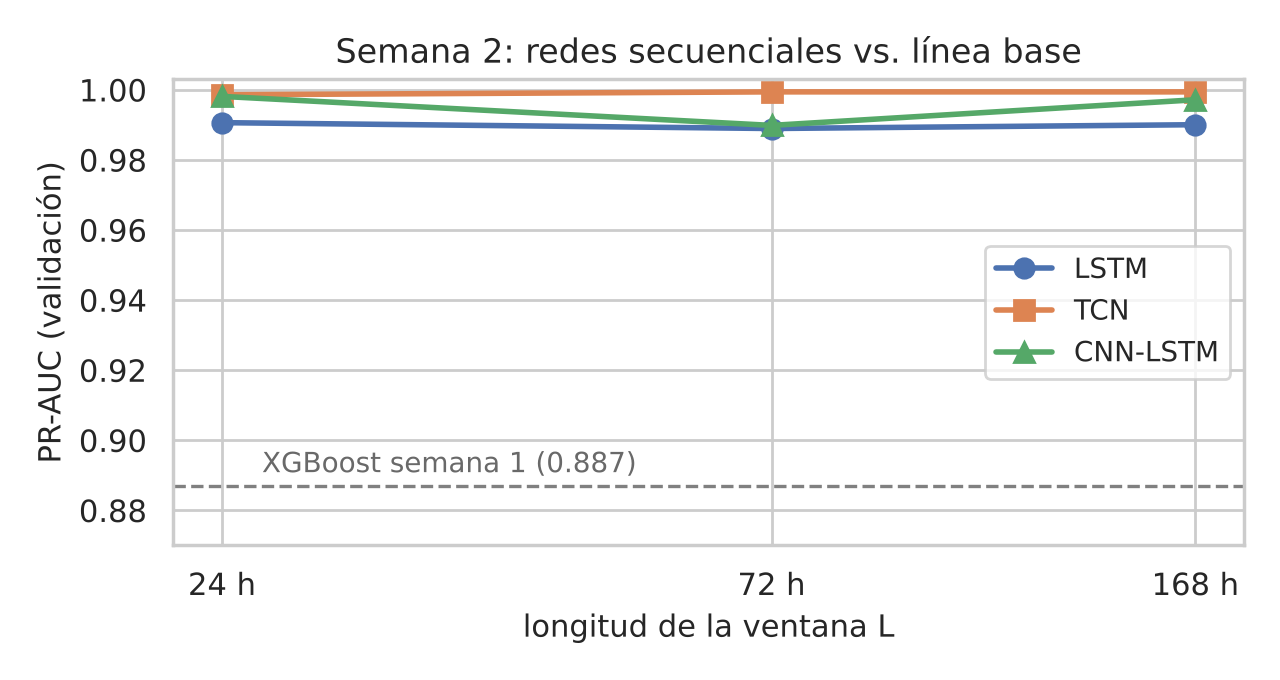
\includegraphics[width=0.9\columnwidth]{figs/week2_effect_L_es.png}
\caption{Semana 2: PR-AUC en validación por arquitectura y longitud de ventana $L$, frente a la línea base XGBoost de la semana 1.}
\label{fig:L}
\end{figure}

\section{Semana 3: modelo avanzado, confiabilidad y política}\label{sec:w3}

\subsection{Transformer con token de máquina}
Cada hora de la ventana se proyecta linealmente a dimensión $d$. Las entradas estáticas (embedding del modelo y antigüedad) se proyectan a un \textit{token de máquina} que se antepone a la secuencia, como el token [CLS] de BERT; se suma codificación posicional sinusoidal~\cite{vaswani}. Dos capas de codificador \textit{pre-norm} con 4 cabezas resumen la ventana, y el estado final del token de máquina, concatenado con el vector estático, alimenta las mismas dos salidas. El entrenamiento es idéntico al de la TCN final ($L=24$, sobremuestreo, $\lambda=0.25$), con un presupuesto declarado de dos tamaños, $d\in\{32,64\}$.

El Transformer con $d=32$ (20\,530 parámetros, 3.4 veces menos que la TCN) alcanzó PR-AUC de 0.9999 en validación, contra 0.9989 de la TCN; con $d=64$ obtuvo 0.9992. Antes de ver los resultados fijamos la regla de selección: gana el menor costo esperado en validación (Sec.~\ref{sec:pol}), y si dos modelos quedan a menos de 1~\%, el más simple. La Tabla~\ref{tab:sel} muestra que los tres candidatos anticipan las 118 fallas de validación y difieren en 0 a 4 falsas alarmas, menos de 1~\% del costo. Se mantiene la TCN de la semana 2. Interpretamos el resultado como saturación: con PR-AUC $\approx 0.999$ en validación, ninguna arquitectura tiene margen para mejorar una decisión que ya es casi perfecta.

\begin{table}[t]
\centering
\caption{Comparación en validación (umbral de precisión $\ge 0.80$ para recall y F1 por componente). $^*$Línea base de las entregas 1--2, con 28 variables construidas; las demás filas usan la serie cruda}
\label{tab:val}
\setlength{\tabcolsep}{3pt}\footnotesize
\begin{tabular}{lcccc}
\toprule
Modelo & PR-AUC & Rec.@P.8 & F1 comp. & Param. \\
\midrule
Reg. logística & 0.850 & 0.838 & 0.768 & --- \\
XGBoost & 0.887 & 0.943 & 0.826 & --- \\
XGBoost, ventanas a mano$^*$ & 0.998 & 1.000 & 0.875 & --- \\
LSTM, $L=24$ & 0.991 & 0.989 & 0.868 & 25k \\
CNN-LSTM, $L=24$ & 0.998 & 1.000 & 0.872 & 37k \\
TCN, $L=24$, submuestreo & 0.999 & 1.000 & 0.868 & 20k \\
TCN + Optuna (final) & 0.999 & 1.000 & 0.866 & 70k \\
Transformer $d=32$ & 1.000 & 1.000 & 0.865 & 21k \\
Transformer $d=64$ & 0.999 & 1.000 & 0.869 & 73k \\
Ensamble 5 TCN & 0.999 & 1.000 & 0.873 & 350k \\
\bottomrule
\end{tabular}
\end{table}

\begin{table}[t]
\centering
\caption{Selección del modelo final por costo en validación (60 días, 118 fallas)}
\label{tab:sel}
\begin{tabular}{lcccc}
\toprule
Modelo & Umbral & Evitadas & F. alarmas & Costo \\
\midrule
TCN (semana 2) & 0.48 & 118 & 3 & 355\,800 \\
Transformer $d=32$ & 0.998 & 118 & 0 & 354\,000 \\
Ensamble 5 TCN & 0.55 & 118 & 4 & 356\,400 \\
\bottomrule
\end{tabular}
\end{table}

\subsection{Incertidumbre y calibración}
\textit{MC Dropout frente a ensamble.} Optuna dejó a la TCN con dropout de 0.023, así que muestrear las máscaras de dropout~\cite{gal} apenas mueve la predicción: con 30 pasadas, la desviación estándar media de $p$ en horas positivas fue de 0.010 en la TCN y de 0.0003 en el Transformer. Por eso estimamos la incertidumbre con un ensamble~\cite{lakshmi} de cinco TCN con la misma configuración y semillas 42--46 (PR-AUC individual de 0.997 a 0.999). El desacuerdo entre miembros resulta informativo: su desviación media es de 0.006 en las alertas correctas y de 0.158 en las horas de falsa alarma, 25 veces mayor. Es una señal útil para pedir una segunda revisión antes de parar una máquina (Sec.~\ref{sec:prod}).

\textit{Calibración.} El sobremuestreo cambia la prevalencia vista en entrenamiento (cerca de 50~\%, contra 1.8~\% real), lo que podría inflar las probabilidades. Ajustamos una temperatura escalar sobre el logit binario minimizando la log-verosimilitud en validación~\cite{guo}; resultó $T=1.15$, casi la identidad. La TCN ya estaba bien calibrada: Brier de 0.00028 y ECE de 0.0001 en validación, con probabilidad media de 0.0185 frente a una prevalencia de 0.0184 (Fig.~\ref{fig:rel}). En prueba, con la temperatura congelada, el Brier fue de 0.00076 y el ECE de 0.0007; la temperatura no cambia el orden de las probabilidades ni, por tanto, las alertas. Estas métricas globales esconden un matiz: el 98~\% de las horas tiene $p<0.1$ y casi todas las demás $p>0.9$, y en las pocas horas intermedias el modelo es sobreconfiado. En prueba, las 210 horas (0.14~\%) con $p$ entre 0.1 y 0.9 tienen una tasa de falla menor que la predicha; por ejemplo, $p\approx0.86$ corresponde a 0.60 observado (Fig.~\ref{fig:reltest}, anexo). Una temperatura única, ajustada en validación donde esas horas casi no aparecen, no lo corrige. En la práctica, la probabilidad intermedia debe leerse como ``riesgo en aumento'' y no como una frecuencia exacta; por eso la alerta exige tres horas sostenidas sobre el umbral. El Transformer muestra el mismo efecto, más marcado, en validación: casi ninguna de sus horas con probabilidad intermedia precedió a una falla (Fig.~\ref{fig:rel}).

\begin{figure}[t]
\centering
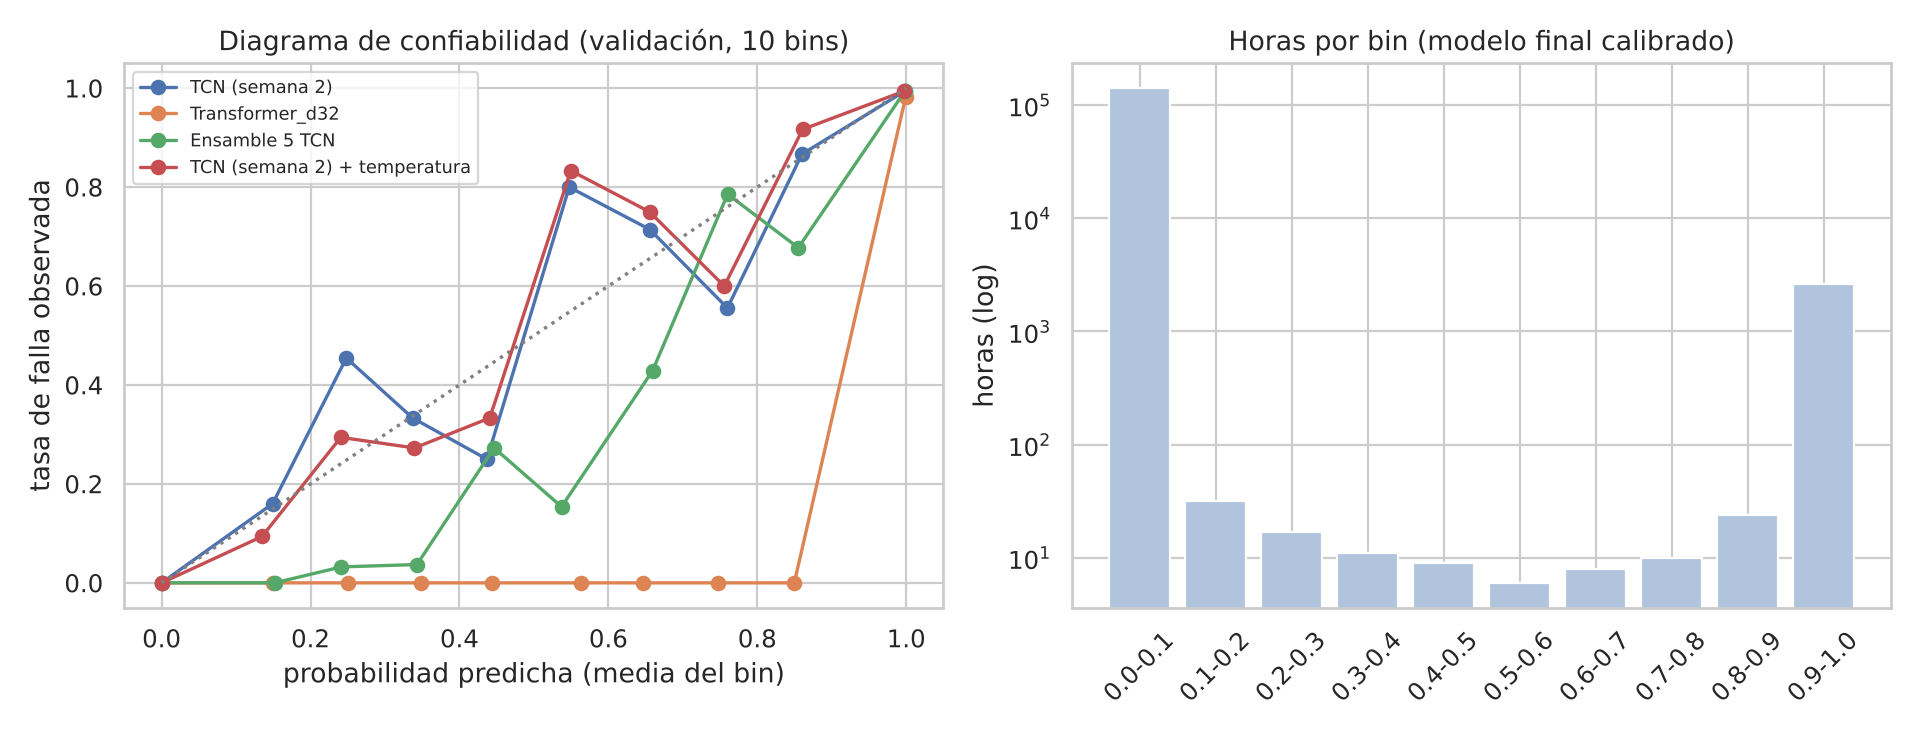
\includegraphics[width=\columnwidth]{figs/reliability_validation.png}
\caption{Diagrama de confiabilidad en validación (izquierda) y número de horas por bin del modelo final calibrado (derecha, escala log).}
\label{fig:rel}
\end{figure}

\subsection{Interpretabilidad}
Aplicamos gradientes integrados~\cite{ig} a la ventana dinámica ($24\times13$), con línea base 0 (la media de entrenamiento de cada canal tras normalizar) y 50 pasos, sobre el logit de la clase $k$, en 200 ventanas de validación que preceden a una falla real de cada componente $k$. La Fig.~\ref{fig:ig} y la Tabla~\ref{tab:ig} muestran un patrón muy limpio: cada componente se explica por un sensor y uno o dos tipos de error, que juntos concentran entre 69 y 74~\% de la atribución. Comp1 se asocia con \textit{volt} y error1; comp2 con error2, error3 y \textit{rotate}; comp3 con \textit{pressure} y error4; y comp4 con \textit{vibration} y error5. La atribución con signo es positiva en todos esos canales para su propio componente y negativa o nula para los demás, es decir, la cabeza multiclase usa esos canales para discriminar entre componentes.

\begin{figure*}[t]
\centering
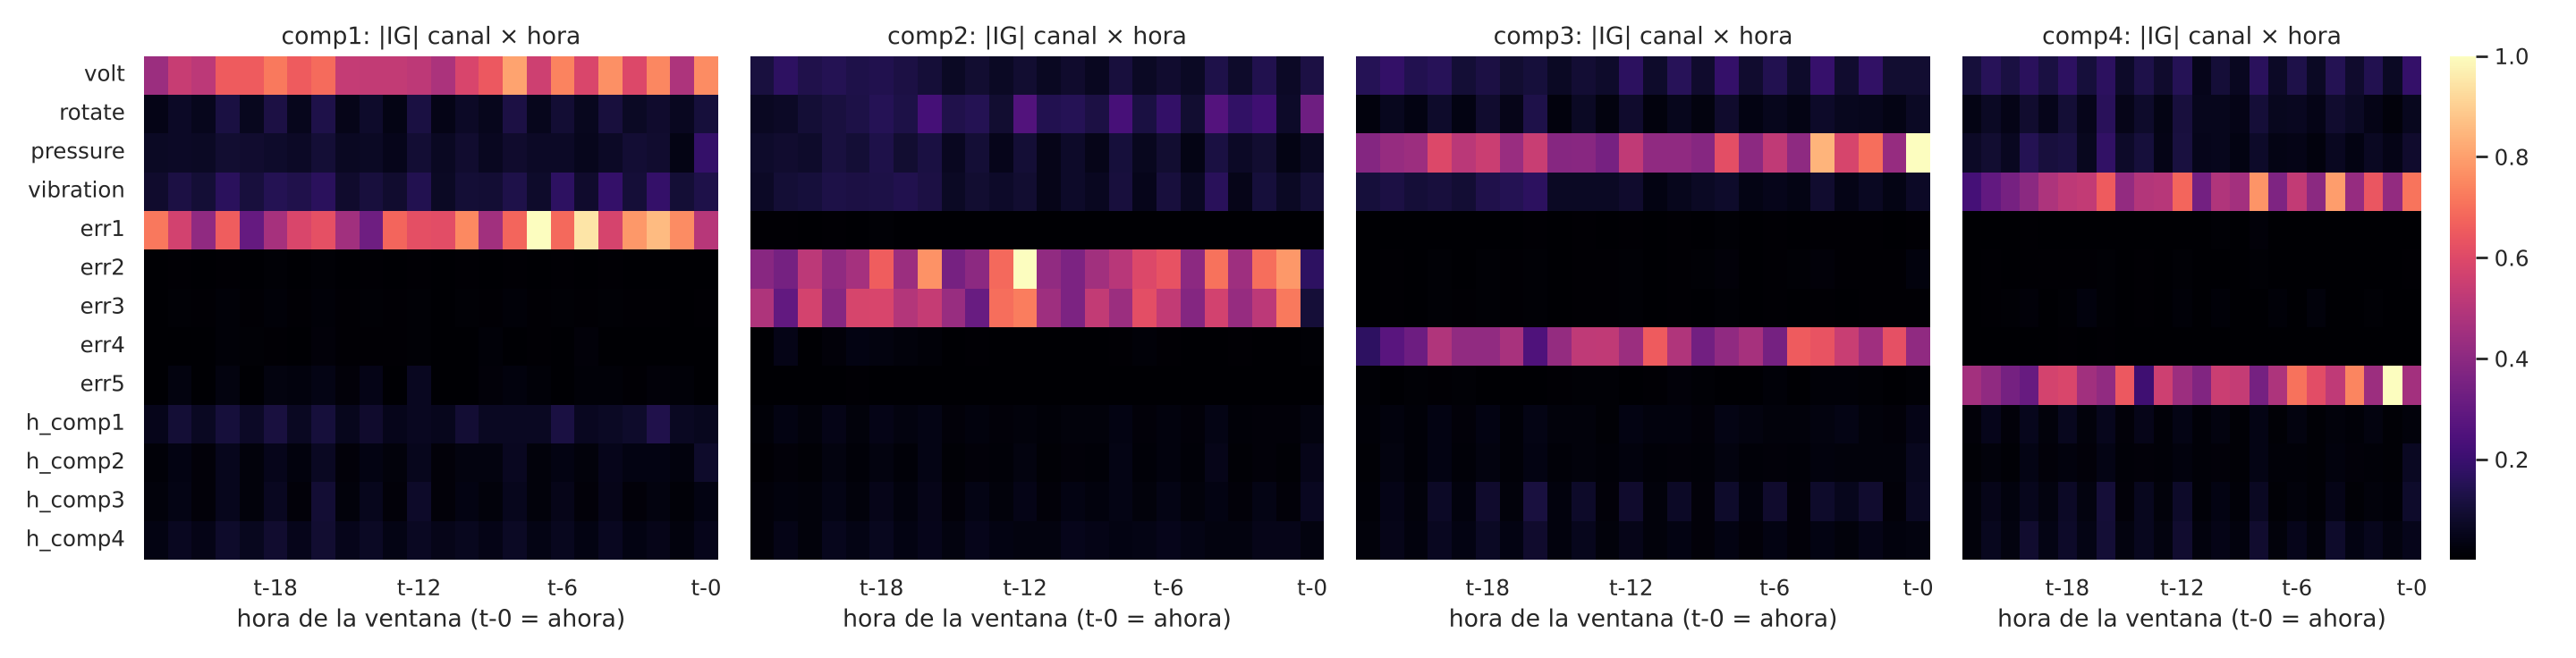
\includegraphics[width=\textwidth]{figs/ig_heatmaps.png}
\caption{Gradientes integrados $|$IG$|$ por canal y hora de la ventana para el logit de cada componente (validación, 200 ventanas pre-falla por componente, normalizado por panel). h\_compk = horas desde el último reemplazo de comp$k$.}
\label{fig:ig}
\end{figure*}

\begin{table}[t]
\centering
\caption{Proporción de $|$IG$|$ por grupo de canales y los tres canales principales}
\label{tab:ig}
\begin{tabular}{lcccl}
\toprule
 & Sensores & Errores & H. reemp. & Top 3 \\
\midrule
comp1 & 0.51 & 0.38 & 0.12 & err1, volt, vibration \\
comp2 & 0.28 & 0.65 & 0.07 & err2, err3, rotate \\
comp3 & 0.56 & 0.34 & 0.10 & pressure, err4, volt \\
comp4 & 0.53 & 0.37 & 0.10 & err5, vibration, volt \\
\bottomrule
\end{tabular}
\end{table}

\textit{Contraste con el análisis exploratorio.} En la semana 1, los errores eran entre 11 y 35 veces más frecuentes en las 24~h previas a una falla que en periodos sanos (de 0.86 a 1.58 por cada 100 horas-máquina, contra 0.03 a 0.10), y los cuatro sensores se desviaban en las 0--48~h previas (por ejemplo, \textit{volt} de 170.6 a 175.9 en promedio y \textit{rotate} de 447.7 a 418.4), mientras que entre 48 y 72~h eran indistinguibles de lo sano. Los gradientes integrados confirman ese hallazgo y lo precisan: el análisis exploratorio mostraba desviaciones agregadas, y el modelo revela que cada componente tiene su propio par sensor--error. El perfil temporal de la atribución se reparte en toda la ventana de 24~h, sin concentrarse en las últimas horas, lo que concuerda con que alargar $L$ no ayudó: la evidencia útil está en el último día. Hay una diferencia relevante con la línea base: en XGBoost, las horas desde el reemplazo eran el grupo dominante, y en la TCN reciben solo entre 7 y 12~\% de la atribución. La red extrae la forma temporal de sensores y errores, que el modelo de rezagos no aprovechaba (solo sensores: PR-AUC 0.34), y por eso depende menos del sustituto ``edad del componente''.

\subsection{Política de mantenimiento}\label{sec:pol}
\textit{Simulación por evento.} Se emite una alerta a la hora $t$ cuando la probabilidad lleva al menos 3 horas seguidas sobre el umbral (la misma definición de alerta sostenida de la semana 2); la decisión se toma en $t$, cuando ya existe la evidencia, y no se emite otra alerta para la misma máquina en las 24~h siguientes. Si alguna falla real de componente ocurre en $(t, t+24\,\text{h}]$, la intervención es acertada: cuesta 3\,000 por componente y la falla se considera evitada. Si no ocurre ninguna, la alerta es una falsa alarma de 600. Una falla sin alerta en las 24~h previas cuesta 15\,000. Contamos fallas por componente para que la política sea comparable con el calendario.

\textit{Umbral.} Barrimos el umbral sobre la probabilidad calibrada en validación (Fig.~\ref{fig:cost}). El costo mínimo forma una meseta entre 0.44 y 0.52; tomamos su mediana, 0.48, para no quedar en el borde. Con ese umbral, en validación se evitan las 118 fallas con 3 falsas alarmas.

\textit{Referencias.} (1) Operar hasta la falla: cada falla cuesta 15\,000. (2) Reemplazo por calendario de cada componente: el componente $k$ se reemplaza (3\,000, intervención planeada) cada vez que su edad llega a $T_k$, sobre la línea de tiempo real de cada máquina. Los reemplazos programados que la planta ya hace siguen ocurriendo en todas las políticas, y una falla real cuenta como evitada si hubo un reemplazo planeado después del último reemplazo real de ese componente. Elegimos $T_k$ minimizando el costo de enero a octubre (el calendario no tiene parámetros entrenados, así que usar entrenamiento y validación da más fallas para elegir sin tocar prueba): 44, 59, 97 y 69 días para comp1 a comp4. Todas las decisiones se congelaron en \texttt{week3\_decisions.json} antes de abrir prueba.

\begin{figure}[t]
\centering
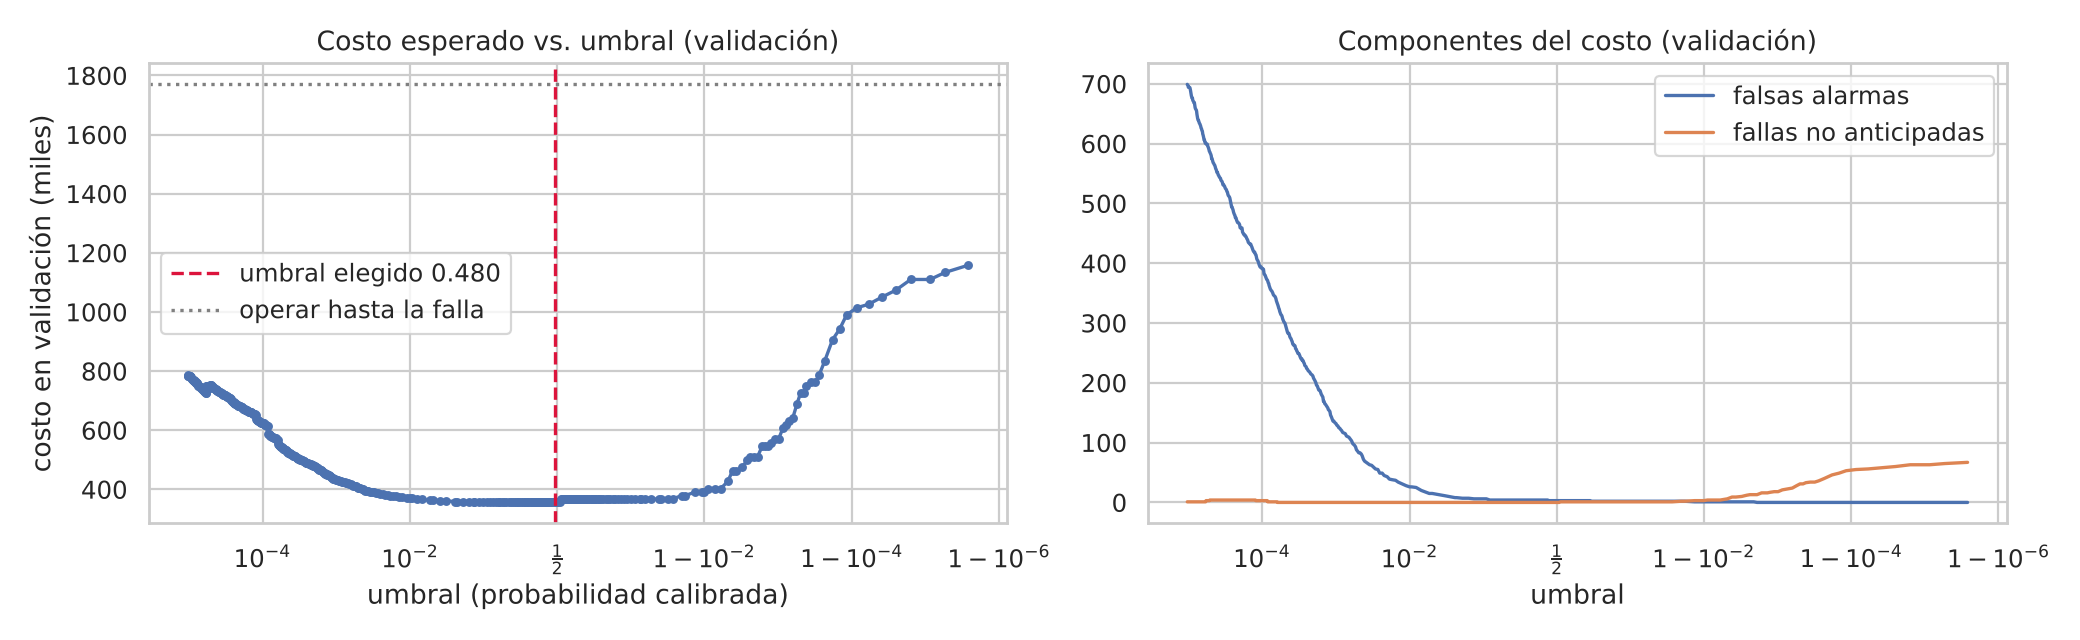
\includegraphics[width=0.95\columnwidth]{figs/cost_vs_threshold.png}
\caption{Costo en validación en función del umbral (eje logit) y sus componentes. La meseta de costo mínimo va de 0.44 a 0.52; el umbral elegido es 0.48.}
\label{fig:cost}
\end{figure}

\section{Resultados en prueba}\label{sec:test}
El conjunto de prueba se evaluó una sola vez, con el modelo, la temperatura, el umbral y los periodos de calendario congelados.

\textit{Métricas del modelo} (Tabla~\ref{tab:test}). PR-AUC de 0.996, ligeramente menor que en validación (0.999), una caída esperable entre periodos distintos. Con el umbral de costo, el 95.8~\% de las horas en alerta precedieron efectivamente a una falla, y se alertó el 99.0~\% de las horas positivas. El F1 macro por componente subió a 0.969, porque el umbral de costo (0.48) es mucho más exigente que el de precisión 0.80 usado en la semana 2 y deja muy pocas horas falsas a las que asignar componente. En las 114 alertas acertadas, la salida multiclase señaló correctamente el componente que falló.

\begin{table}[t]
\centering
\caption{Modelo final (TCN) en prueba, noviembre--diciembre de 2015}
\label{tab:test}
\begin{tabular}{lc}
\toprule
Métrica & Prueba \\
\midrule
PR-AUC / ROC-AUC & 0.996 / 1.000 \\
Recall con precisión $\ge 0.80$ & 1.000 \\
Precisión / recall por hora (umbral 0.48) & 0.958 / 0.990 \\
F1 macro comp1--comp4 (umbral 0.48) & 0.969 \\
F1 por componente & 0.95 / 1.00 / 0.94 / 0.99 \\
Fallas con alerta sostenida & 121 de 121 \\
Aviso medio antes de la falla & 21.0 h \\
Componente correcto en alertas acertadas & 114 de 114 \\
Brier / ECE (con temperatura) & 0.00076 / 0.0007 \\
\bottomrule
\end{tabular}
\end{table}

\textit{Costo de las tres políticas} (Tabla~\ref{tab:cost}). En los 61 días de prueba, la política del modelo emitió 126 alertas: 114 acertadas, que cubrieron las 121 fallas, y 12 falsas alarmas, es decir, 1.4 por semana para la flota de 100 máquinas. Su costo anualizado es de 2.2 millones, 80~\% menos que operar hasta la falla (10.9 M) y 74~\% menos que el calendario (8.4 M). Para dimensionar la incertidumbre por el número limitado de fallas, remuestreamos las 100 máquinas con reemplazo (2\,000 réplicas, la misma muestra para las tres políticas). Los intervalos de 95~\% son 1.9--2.5 M para el modelo, 7.2--9.6 M para el calendario y 9.2--12.5 M para operar hasta la falla. El ahorro del modelo es de 8.6 M (7.3--9.9) frente a operar hasta la falla y de 6.1 M (5.2--7.2) frente al calendario; ningún intervalo de ahorro incluye el cero. El calendario evita 73 de 121 fallas, pero a cambio de 226 reemplazos planeados, muchos de piezas que no iban a fallar. Los resultados de prueba reproducen los de validación (2.16, 8.19 y 10.77 M), lo que indica que el umbral no quedó sobreajustado.

\begin{table}[t]
\centering
\caption{Costo anual estimado (millones; flota de 100 máquinas; periodo $\times$ 365/días). IC: bootstrap por máquina}
\label{tab:cost}
\setlength{\tabcolsep}{3pt}\small
\begin{tabular}{llccccc}
\toprule
 & Política & Evit. & No antic. & F. al. & M/año & IC 95\,\% \\
\midrule
\multirow{3}{*}{Valid.} & Hasta la falla & 0 & 118 & 0 & 10.77 & \\
 & Calendario & 71 & 47 & --- & 8.19 & \\
 & Modelo & 118 & 0 & 3 & 2.16 & \\
\midrule
\multirow{3}{*}{Prueba} & Hasta la falla & 0 & 121 & 0 & 10.86 & 9.2--12.5 \\
 & Calendario & 73 & 48 & --- & 8.37 & 7.2--9.6 \\
 & Modelo & \textbf{121} & \textbf{0} & 12 & \textbf{2.22} & 1.9--2.5 \\
\bottomrule
\end{tabular}
\end{table}

\textit{Sensibilidad.} Fijamos la falsa alarma en 600 y la intervención acertada en 3\,000, y variamos la falla no anticipada como $r\times600$ con $r\in\{5,10,15,25,50,100\}$. Para cada $r$, re-elegimos el umbral en validación y $T_k$ en enero--octubre (con una rejilla de 48~h, por eso el calendario base difiere en 0.2~\% de la Tabla~\ref{tab:cost}) y evaluamos en prueba (Fig.~\ref{fig:sens}). Con $r=5$, una falla cuesta lo mismo que intervenirla y ninguna política ahorra. Desde $r=10$, el modelo es la mejor opción y su punto de operación no cambia (umbral 0.48, 1.4 falsas alarmas por semana, 100~\% de fallas evitadas), así que su costo queda fijo en 2.2 M mientras el de las otras políticas crece con $r$. El calendario solo supera a operar hasta la falla a partir de $r\approx15$. La conclusión es robusta: el modelo conviene siempre que una falla cueste al menos el doble que una intervención planeada.

\begin{figure}[t]
\centering
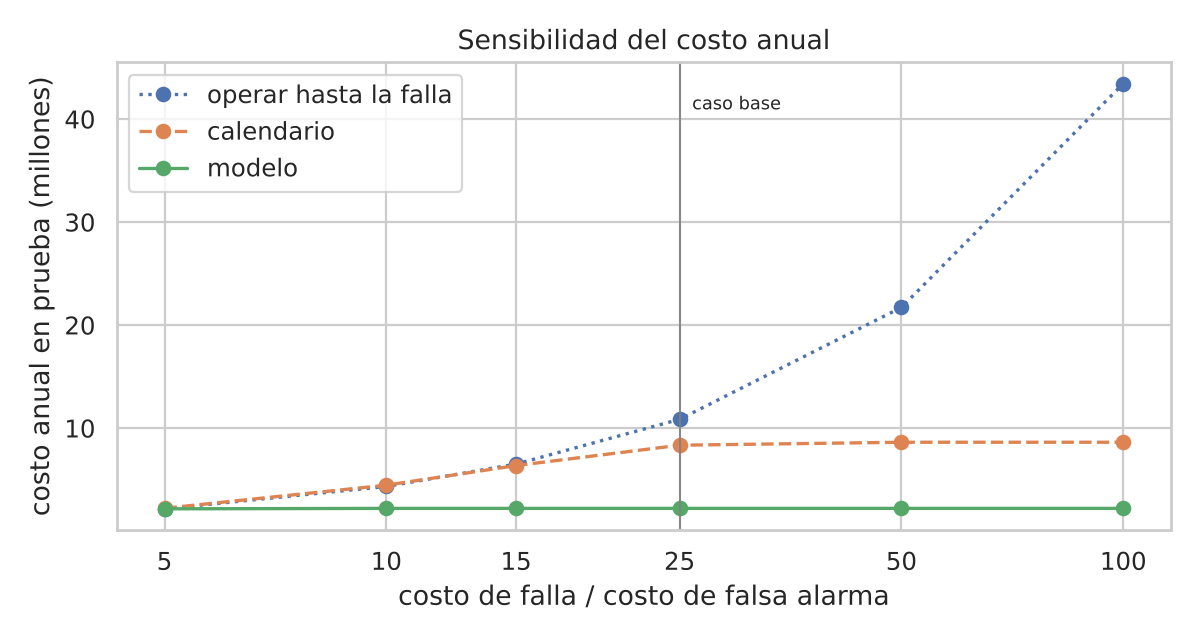
\includegraphics[width=0.9\columnwidth]{figs/sensitivity.png}
\caption{Costo anual en prueba de las tres políticas al variar la razón entre el costo de falla y el de falsa alarma (umbral y $T_k$ re-elegidos sin usar prueba para cada razón).}
\label{fig:sens}
\end{figure}

\section{Discusión}\label{sec:disc}
\textit{¿Supera el deep learning a la línea base?} Depende de la entrada. Con la misma serie cruda, sí y con margen: XGBoost llega a PR-AUC de 0.887 y la TCN a 0.999. Con las variables de ventana diseñadas a mano en las entregas 1--2, XGBoost empata (0.998). La ablación y los gradientes integrados explican por qué. La señal está en la forma temporal de sensores y errores dentro del último día: las convoluciones causales la capturan directamente, mientras que un modelo de árboles necesita que alguien la resuma en medias y conteos de 24~h. La ventaja real de la red es, entonces, no depender de ese diseño de variables, lo que importa en una planta real, donde no se sabe de antemano qué ventanas ni qué estadísticos son los relevantes. A cambio, un XGBoost con buenas variables es más barato de entrenar y más fácil de explicar, y en este conjunto rinde lo mismo. Entre las redes, en cambio, las diferencias son irrelevantes para la decisión: el Transformer, más moderno y con menos parámetros, empata con la TCN en costo. Preferimos el modelo más simple ya validado y lo declaramos así antes de mirar.

\textit{Anticipación.} El aviso medio de 21~h está acotado por diseño: la etiqueta define un horizonte de 24~h, el modelo aprende a encender la alerta al entrar en esa ventana, y la alerta sostenida exige tres horas. Avisos con varios días de anticipación requerirían entrenar con un horizonte mayor (por ejemplo, 72~h o un modelo de tiempo hasta la falla) y aceptar más falsas alarmas.

\textit{Datos simulados.} El conjunto es didáctico y sus patrones son más limpios que en una planta real: cada componente se asocia con un sensor y unos tipos de error concretos, las fallas se registran a horas fijas (06:00 o 03:00) y no hay datos faltantes. Con datos reales esperaríamos deriva de sensores (que exigiría normalización móvil y reentrenamiento), huecos de telemetría, registros de mantenimiento incompletos o tardíos (que afectan directamente las horas desde el reemplazo) y errores con causas múltiples. Las cifras de este reporte deben leerse como el techo de lo alcanzable, no como una promesa.

\section{Limitaciones y camino a producción}\label{sec:prod}
\textit{Limitaciones.} (i) La prueba cubre 61 días y 121 fallas; con tan pocos eventos, 12 falsas alarmas frente a 3 en validación está dentro de la variación esperable, y las cifras anuales son extrapolaciones (los intervalos bootstrap cuantifican la variación entre máquinas, no la estacionalidad). (ii) El calendario es un contrafactual: suponemos que un reemplazo planeado elimina la falla del componente desgastado y que el nuevo no falla dentro del mismo periodo. (iii) Los costos son los del enunciado y suponemos que un reemplazo planeado cuesta lo mismo que una intervención acertada. (iv) El modelo se eligió con una métrica saturada; con datos reales, las diferencias entre arquitecturas podrían reaparecer. (v) Las probabilidades intermedias son sobreconfiadas, aunque corresponden a muy pocas horas.

\textit{Para producción} se necesitaría: (1) un flujo de datos horario confiable desde el controlador y el sistema de mantenimiento, con reglas para datos faltantes; (2) un piloto en modo sombra de 2 a 3 meses, en el que el modelo alerte sin detener máquinas y se registre qué habría pasado; (3) los costos reales de la planta para recalcular el umbral; (4) monitoreo de deriva y de la tasa de falsas alarmas, con reentrenamiento periódico; (5) usar el desacuerdo del ensamble como semáforo, mandando a inspección rápida las alertas inciertas en lugar de parar la máquina; y (6) un modelo complementario con horizonte mayor para planear refacciones y personal.

\section{Conclusiones}
Construimos y evaluamos de punta a punta un sistema de alerta temprana con etiquetas sin fuga, partición temporal estricta y un único uso del conjunto de prueba. La TCN con ventana de 24~h anticipó las 121 fallas del periodo de prueba con 21~h de aviso medio y 1.4 falsas alarmas por semana, y reduce el costo estimado de 10.9 a 2.2 millones al año, frente a 8.4 millones del reemplazo por calendario. Las probabilidades están bien calibradas en conjunto, aunque son sobreconfiadas en las pocas horas de riesgo intermedio; la atribución coincide con la física aparente del conjunto y su ventaja se mantiene en todo el análisis de sensibilidad siempre que una falla cueste más que su intervención.

\begin{thebibliography}{9}
\bibitem{azure} Microsoft, ``Predictive Maintenance Modelling Guide,'' Azure AI Gallery, 2016.
\bibitem{bai} S.~Bai, J.~Z.~Kolter y V.~Koltun, ``An empirical evaluation of generic convolutional and recurrent networks for sequence modeling,'' arXiv:1803.01271, 2018.
\bibitem{lstm} S.~Hochreiter y J.~Schmidhuber, ``Long short-term memory,'' \textit{Neural Computation}, vol.~9, no.~8, pp.~1735--1780, 1997.
\bibitem{vaswani} A.~Vaswani \textit{et al.}, ``Attention is all you need,'' en \textit{Proc. NeurIPS}, 2017.
\bibitem{gal} Y.~Gal y Z.~Ghahramani, ``Dropout as a Bayesian approximation: Representing model uncertainty in deep learning,'' en \textit{Proc. ICML}, 2016.
\bibitem{lakshmi} B.~Lakshminarayanan, A.~Pritzel y C.~Blundell, ``Simple and scalable predictive uncertainty estimation using deep ensembles,'' en \textit{Proc. NeurIPS}, 2017.
\bibitem{guo} C.~Guo, G.~Pleiss, Y.~Sun y K.~Q.~Weinberger, ``On calibration of modern neural networks,'' en \textit{Proc. ICML}, 2017.
\bibitem{ig} M.~Sundararajan, A.~Taly y Q.~Yan, ``Axiomatic attribution for deep networks,'' en \textit{Proc. ICML}, 2017.
\bibitem{focal} T.-Y.~Lin \textit{et al.}, ``Focal loss for dense object detection,'' en \textit{Proc. ICCV}, 2017.
\end{thebibliography}

\clearpage
\appendices
\section{Reproducibilidad}
{\raggedright
El repositorio incluye \texttt{requirements.txt} y usa semilla 42. Orden de ejecución:
\begin{enumerate}
\item {\footnotesize\texttt{week1\_predictive\_maintenance\_serie\_cruda.ipynb}}\\ datos, etiquetas, partición y línea base.
\item {\footnotesize\texttt{week2\_deep\_learning\_baselines\_week1.ipynb}}\\ redes secuenciales y \texttt{models/week2\_best.pt}.
\item {\footnotesize\texttt{week3\_advanced\_reliability\_policy.ipynb}}\\ Transformer, ensamble, calibración, gradientes integrados, política y prueba.
\end{enumerate}
Las redes de la semana 3 se guardan en \texttt{models/week3/}; \texttt{train\_week3.py} las entrena con los mismos argumentos que el notebook. En CPU de 2 núcleos, cada Transformer tardó de 2 a 4 minutos y cada TCN del ensamble de 2 a 3.5 minutos.

\textit{Decisiones congeladas antes de abrir prueba} (\texttt{data/processed/week3\_decisions.json}): modelo final TCN de la semana 2; temperatura 1.154; umbral 0.48; alerta sostenida de 3~h con enfriamiento de 24~h; $T_k$ = 1\,056, 1\,416, 2\,328 y 1\,656~h.

\textit{Nota sobre el modelo de la semana 2.} Los pesos guardados en \texttt{models/week2\_best.pt} corresponden al ensayo 3 de Optuna (dropout 0.023, $\lambda=0.25$, lr $1.3\times10^{-3}$, 64 canales); la salida impresa en el notebook de la semana 2 es de una ejecución anterior. La semana 3 verifica que los pesos reproducen las predicciones guardadas (diferencia máxima de $9\times10^{-7}$).\par}

\section{Figuras adicionales}
\begin{figure}[h]
\centering
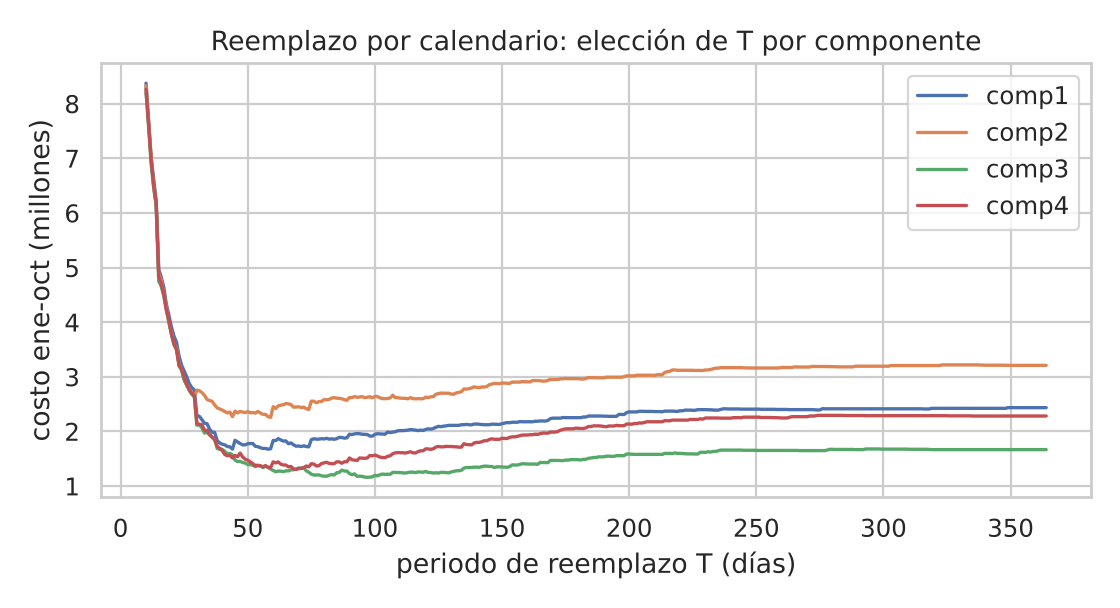
\includegraphics[width=\columnwidth]{figs/calendar_T.png}
\caption{Elección del periodo de reemplazo por calendario $T_k$ (costo de enero a octubre).}
\end{figure}
\begin{figure}[h]
\centering
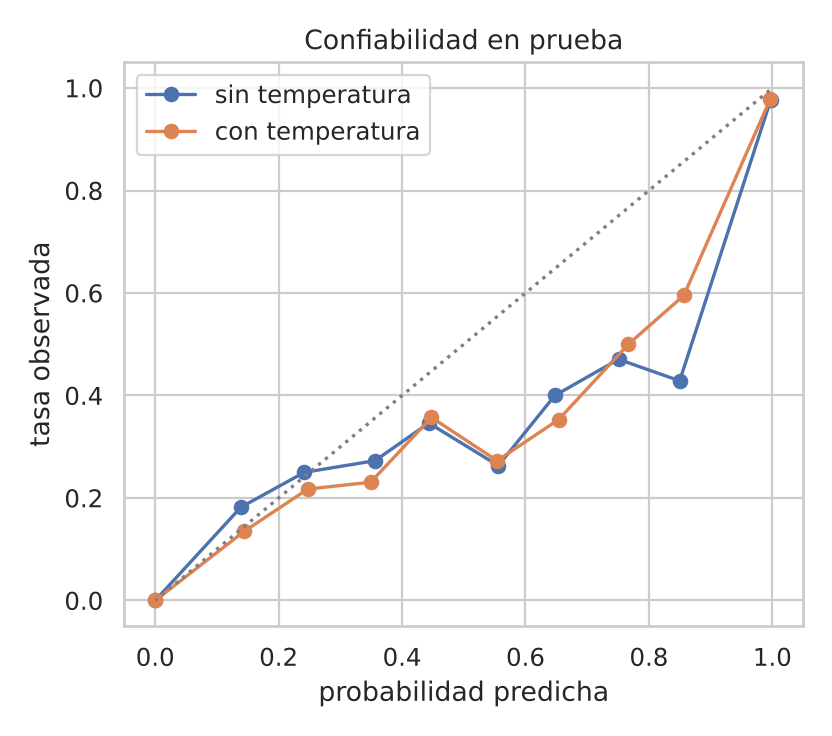
\includegraphics[width=\columnwidth]{figs/reliability_test.png}
\caption{Confiabilidad en prueba con y sin temperatura (10 bins; los bins entre 0.1 y 0.9 reúnen solo 210 horas).}\label{fig:reltest}
\end{figure}
\begin{figure*}[h]
\centering
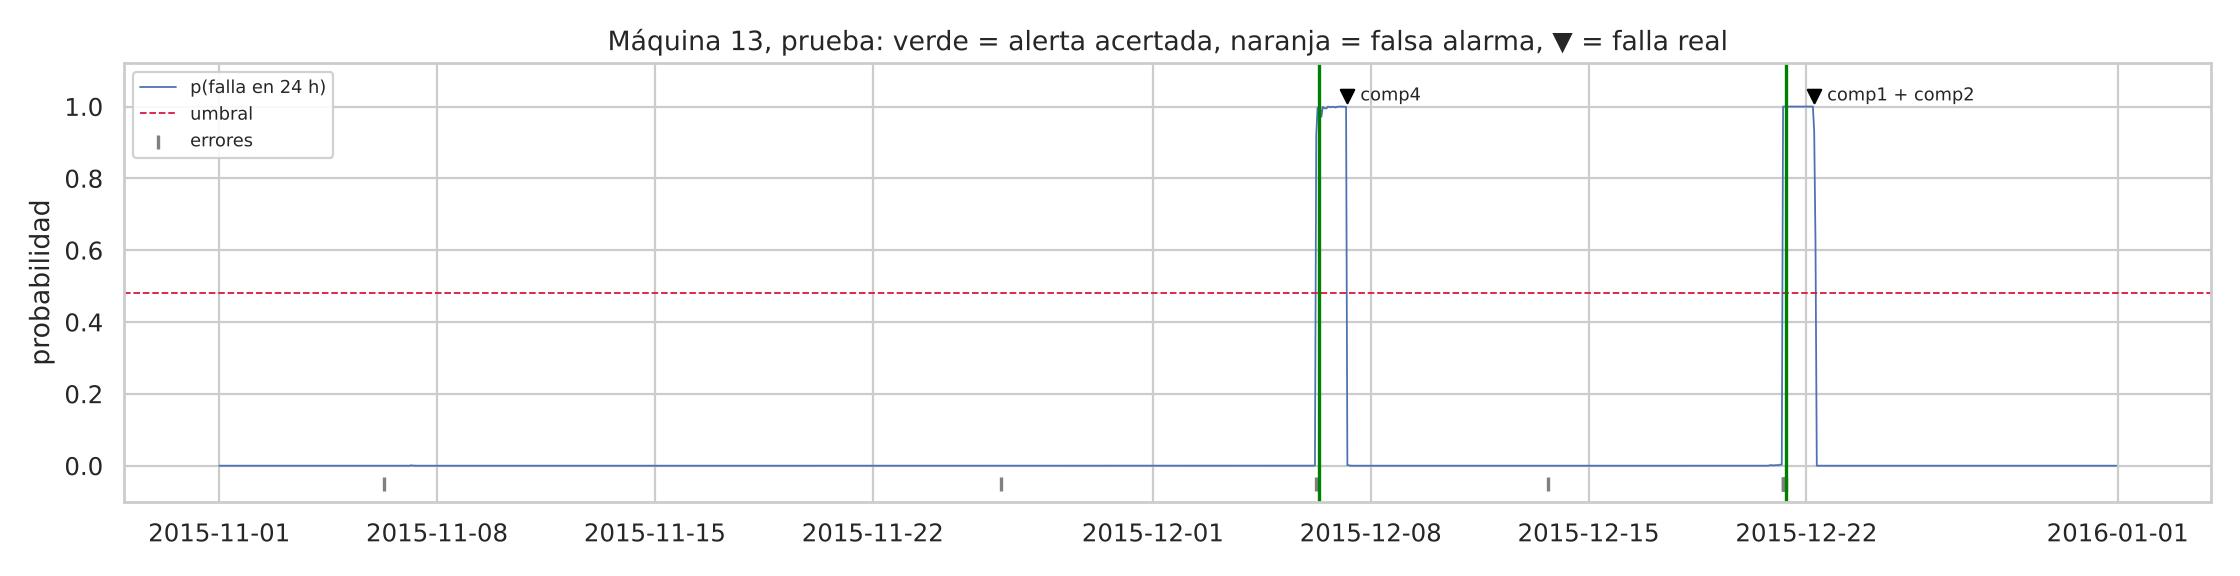
\includegraphics[width=\textwidth]{figs/machine_check_test.png}
\caption{Revisión a mano de la máquina 13 en prueba: probabilidad del modelo, umbral, alertas (verde: acertada) y fallas reales.}
\end{figure*}
\begin{figure}[h]
\centering
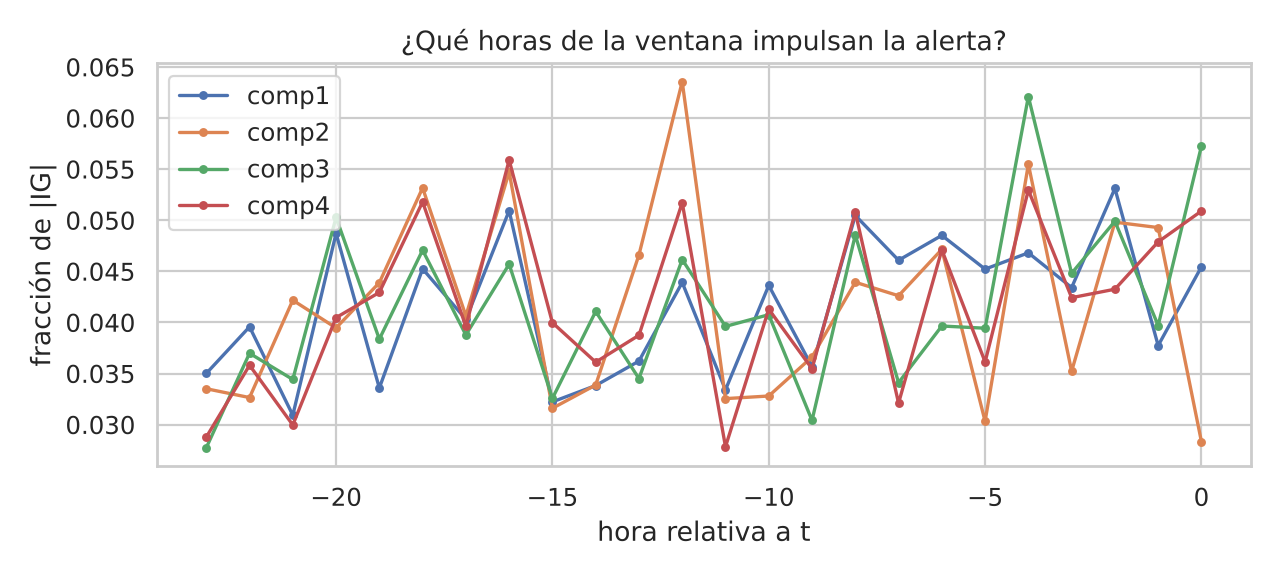
\includegraphics[width=\columnwidth]{figs/ig_time_profile.png}
\caption{Proporción de la atribución por hora de la ventana para cada componente.}
\end{figure}
\begin{figure}[h]
\centering
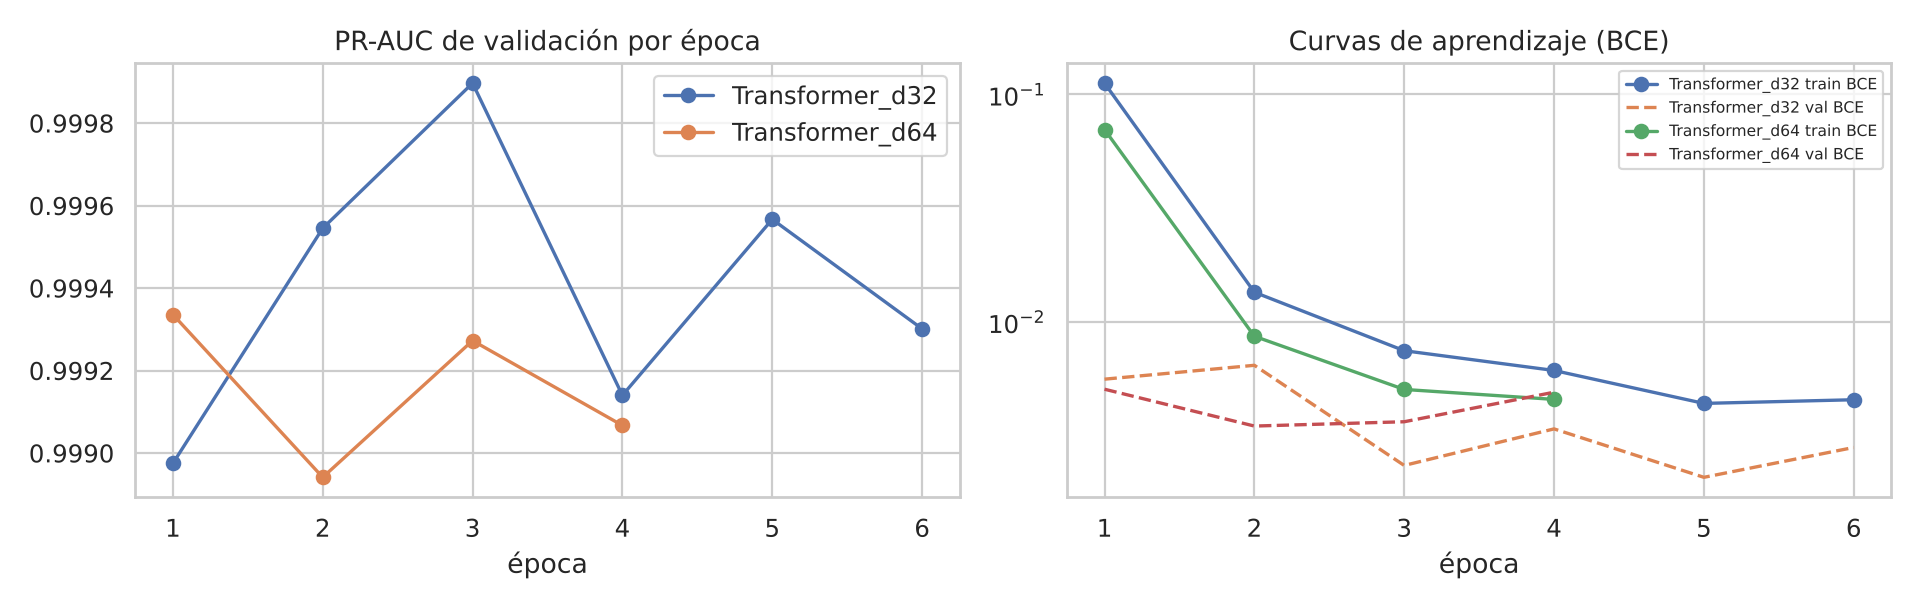
\includegraphics[width=\columnwidth]{figs/transformer_learning_curves.png}
\caption{Curvas de aprendizaje de los dos Transformers.}
\end{figure}

\end{document}
